\graphicspath{{../images/ch4/}}	% Image directory


\chapter{Resistive pulse studies of aspherical mesoparticles}
\label{chap:rods}
	

	\section{Background \& Theory}
		In the introduction of this dissertation we introduced and explained the theory behind resistive pulse sensing, a particle characterization technique that works by monitoring the change in conductance of a nanopore as small particles pass through it. Probably the most important application of RP sensing is in measuring the sizes of particles. An analytic model was devised by DeBlois \emph{et al.} to relate the size of a particle to its resistive pulse amplitude. The solution is essentially an electrostatics boundary-value problem: given an insulating particle inside a pore and a known externally applied voltage, calculate the electric field distribution inside the pore, and from the electric field distribution calculate the pore's expected resistance with the particle inside it. When this calculation is performed for spherical particles travelling along the axis of long cylindrical pores, the change in resistance or current is found to be
		
		\begin{equation}\label{eq:dI}
			\frac{\Delta R}{R_{0}}=\frac{\Delta I}{I_{p}}=\frac{4\rho D^{3}}{\pi d^{4}}\left[1-0.8\left(\frac{d}{D}\right)^{3}\right].
		\end{equation}
		
		Equation \ref{eq:dI} is useful for relating the change in current---or resistance---to the diameter of spherical particles. However, it is very often the case that particles of interest are not spherical. For instance, many biomolecules such as viruses and proteins are poorly approximated as spheres, and are more rod-like in shape. In this case, the resistive pulse amplitude of on-axis translocations through a cylindrical pore is given by 
		
		\begin{equation}\label{eq:dIellipsoid}
			\frac{\Delta R}{R_{0}}=\left[f_{\perp}+\left(f_{\parallel}-f_{\perp}\cos^{2}\alpha\right)\right]\frac{v}{V},
		\end{equation}

		where $f_{\perp}$ and $f_{\parallel}$ are so called `shape-factors', that depend on the particle's major and minor axis lengths, $\alpha$ is the orientation of the particle with $\alpha=0$ being axially aligned, and $v$ and $V$ are the volume of the particle and of the pore, respectively. Figure \ref{fig:dIellipsoid} shows a plot of the relative $\Delta I/I_{p}$ for various ellipsoids of the same volume but different axial lengths.
		
		\begin{figure}
			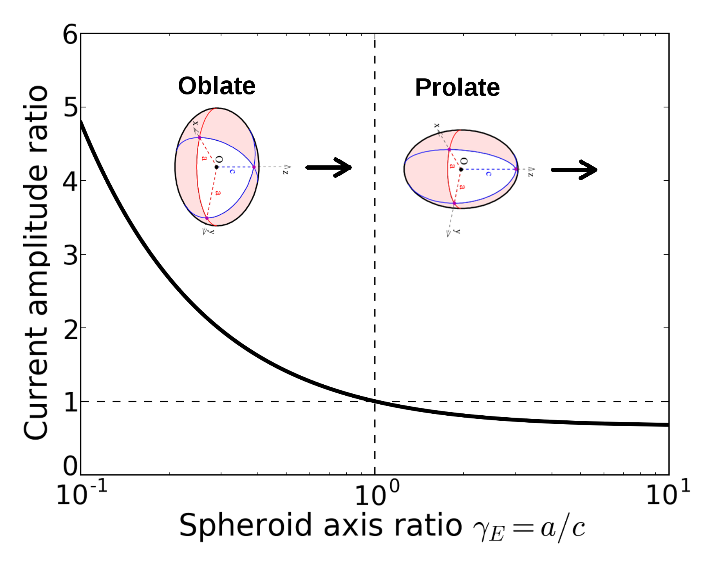
\includegraphics[width=0.5\textwidth]{dIellipsoid}
			\caption{adsf}
			\label{fig:dIellipsoid}
		\end{figure}

		
		
		
		
		
		
		While equation \ref{eq:dIellipsoid} is useful for determining the volume of spheroidal particles from their resistive pulse amplitudes, it would be useful to devise a method for measuring the length of particles in addition to measuring their volumes as an additional physical marker for their identification in a sample.
		
		Consider a pore with a rough, non-uniform interior. Due to the irregular interior, the channel cross sections will have a range of resistance values; for instance, a large cavity in the channel will have a smaller resistance than a more narrow constriction. If a very small particle travels through the pore, its resistive pulse time-series is determined by the interior topology of the pore. For instance, when it happens to occupy a narrower region of the pore, the resistance in tha tregion is larger relative to the rest of the pore, and therefore the particle  will also block a relatively larger portion of the current. In this way, the particle is able to resolve the interior features of the pore. In such cases, the instantaneous resistive pulse amplitude is given by 
		
		\begin{equation}\label{eq:dIlocal}
			\Delta R=R_{p}-R_{0}=\frac{4\rho d^{3}}{\pi D^{4}}\left[1-0.8\left(\frac{d}{D}\right)^{3}\right]^{-1}.
		\end{equation}

		
		\begin{equation}\label{eq:theoreticalmovingaverage}
			\Delta R=\Delta R'=\int_{z=z'}^{z=z'+l}\frac{d\Delta R\left(z\right)}{dz}\,dz=\int_{z=z'}^{z=z'+l}\frac{4\rho d^{3}}{\pi D^{4}\left(z\right)}\left[1-0.8\left(\frac{d}{D\left(z\right)}\right)^{3}\right]^{-1}\,dz
		\end{equation}

		
		Oppositely, if we consider a pore whose length extends along a significant amount of the pore's axis, it may be occupying several such regions at a time. Instead of a single particle, we may consider the particle to be composed of many smaller segments of particles in series, and therefore the resistance values of each segment are additive. Therefore, the signals of longer particles can be seen as the convolution of the signal of an infinitesimally small particle over the long particle's length. 
		
		This fact can be used to devise an experiment that can measure the length of long particles. First, we drive a suspension of small `tracer' spheres through a pore with rough interior, whose diameter is smaller than the characteristic length of the irregularities in the pore. These particles will `map' the interior geometry of the pore as explained above, with resistive pulse shape given by equation \ref{eq:dIlocal}. Then, we repeat the experiment with long particles for which we wish to know the length. Then we perform a convolution or moving average transformation of the signals of the tracer particles for a variety of lengths, given by the following equations:
		
		\begin{equation}\label{eq:movingaverage}
			I_{i}\rightarrow I_{i}^{l'}=\frac{1}{N}\Sigma_{j=i-\frac{N}{2}}^{j=i+\frac{N}{2}}I_{j}, \mathrm{and} \\
			N=\frac{fl'}{v},
		\end{equation}
		
		where N is the total number of points in the moving average, $I_{i}$ is the $i$th current measurement in the signal of the unprocessed short particle, $I_{i}^{l'}$ is the transformed data point for a moving average over length $l'$, $f$ is the sampling frequency of the current acquisition instrument, and $v$ is the \textit{average} velocity of the particle during its translocation through the pore. However, equation \ref{eq:movingaverage} slightly oversamples particle positions in the middle of the moving average compared to particle positions at the very ends, along a distance equal to half the length of the small particle. For this reason, the moving average estimate of the correct transformation slightly overestimates the length of long particles. However, when $l\ll l'$, i.e. the tracer particle's displacement length is much less than the longer rod's displacement length, the effect is negligibly small. 

		
		After computing the moving averages of the tracer particles over an array of lengths, a similarity measure is calculated between every pair of convoluted-raw signals for the tracer particle and the long particle, and the length with the greatest similarity measure is chosen as the correct length of the particle.
		
		Probably the simplest similarity measure of two time-series is the point-wise summed Euclidean distance between the two signals given by the following formula:
		
		\begin{equation}\label{eq:euclideandistance}
			C\left(S, S'\right)=\Sigma_{i=0}^{N-1}\left(S_{i}-S'_{i}\right).
		\end{equation}
		
		\begin{figure}
			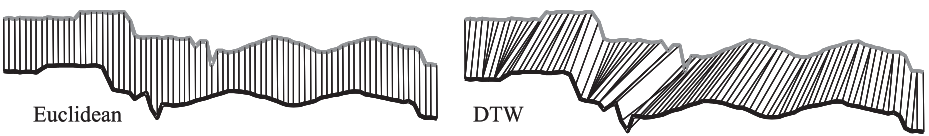
\includegraphics[width=\textwidth]{eucliddtw}
			\caption{\textbf{Comparison of standard Euclidean distance metric (left) and distance metric as determined by dynamic time warping (right).} Notice that the Euclidean distance does not take into account small displacements of the two signals in time, despite their obvious similarity. On the other hand, dynamic time warping is able to account for small mismatches in time by finding the connections between points that minimizes the total cost.}
			\label{fig:eucliddtw}
		\end{figure}

		
		However, the problem with this similarity measure is it is not robust against small variations in the phases of the two signals, i.e. if the two signals evolve in time noisily such that they are not instantaneously exactly in phase. For instance, Fig. \ref{fig:eucliddtw}A shows two resistive pulse time-series taken during an experiment and overlapped exactly in time, with lines connecting the points that would be summed in the Euclidean distance metric\cite{Keogh2005}. Notice that the two sequences are very similar, but due to a non-perfect alignment of identical features in time, the aligned Euclidean distance metric will greatly penalize the similarity of the two signals. One method of measuring the similarity of two time-series that accounts for time offsets is dynamic time warping.
		
		\subsection{Dynamic time warping}
		
			Figure \ref{fig:eucliddtw}B shows two time-series signals that have been aligned after dynamic time warping. The image shows that the algorithm is capable of matching points that are not perfectly aligned in time, but that reflect the actual progression of the two signals in synchronization. The algorithm works as follows.
			
			\begin{figure}
				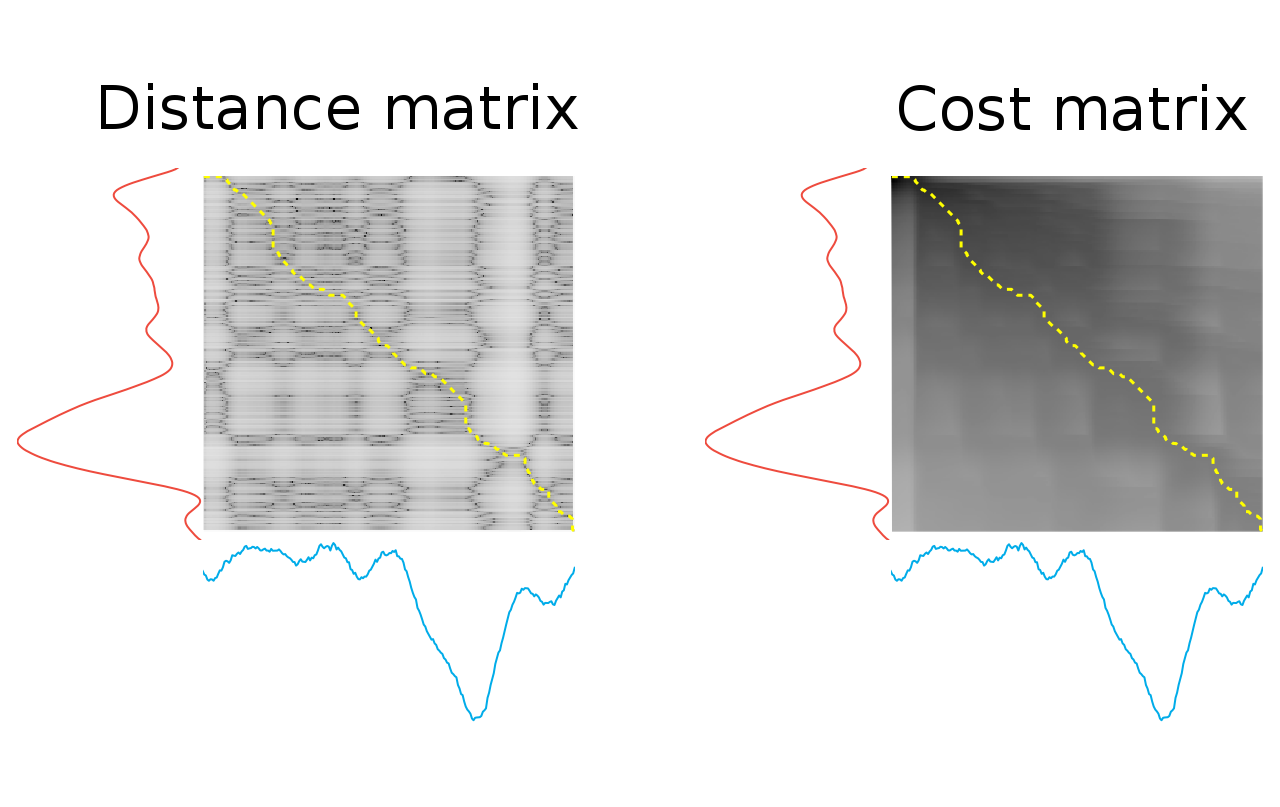
\includegraphics[width=\textwidth]{distancecost}
				\caption{\textbf{Distance (left) and cost matrices (right) of two resistive pulse signals as determined by dynamic time warping.} The element $\left(i,j\right)$ in the distance matrix represents the Euclidean distance between the two signals, $\left(S_{i}-S'_{j}\right)^{2}$. Every element in the cost matrix represents the summed Euclidean distance along the minimum path that arrives at that point. Therefore, the point at the lower right-most point in the distance matrix is the summed cost to completely connect the two signals. The path that yields the cost of that element in the matrix is represented by the yellow dashed line.}
				\label{fig:distancecost}
			\end{figure}

			
			First, a matrix $D_{i,j}$ of the point-wise Euclidean distance between all two points in the two signals is created, as shown in Fig. \ref{fig:distancecost} (left). For instance, point $D_{3,4}$ is the Euclidean distance between point $3$ and $4$ in signals $S$ and $S'$, respectively. The objective is to traverse through the distance matrix along the path that minimizes the total accumulated distance, or the cost $C$, subject to certain kinematic constraints, described below. Each step in the trajectory is defined by the indices from the two respective signals $\left(i,j\right)$. The non-warped Euclidean distance metric given by Eq. \ref{eq:euclideandistance} would correspond to a straight diagonal trajectory through the matrix, e.g. no warping at all. Although there are several formulations of dynamic time warping, the original method only allows for three types of motion such that $\left(i,j\right)\rightarrow\left(i+1,j\right)$ (progressive vertical motion), $\left(i,j\right)\rightarrow\left(i+1,j+1\right)$ (progressive diagonal motion), or $\left(i,j+1\right)$ (progressive horizontal motion). Regressive motion, which would correspond to taking a step backwards in the path back towards the upper left cell in the matrix, is forbidden. The key to dynamic time warping is the means by which we determine the optimal path that minimizes the total accumulated distance. The problem is combinatorically large and scales like $2^{\sqrt NN'}$, where $N, N'$ are the number of data points in each of the two signals. Due to this scaling, random searching of paths through the matrix is not a feasible means of determining the optimum path for large $NN'$. As the name implies, dynamic time warping implies a dynamic computational algorithm for determining the minimum path, described as follows. First, we must recognize that, due to the rules for stepping through the matrix, the minimum path to arrive at point $\left(i,j\right)$ must pass through one of points $\left(i-1,j\right)$, $\left(i-1,j-1\right)$, or $\left(i,j-1\right)$. Therefore, the cost $C$ of point $\left(i,j\right)$ is given by
			
			\begin{equation}\label{eq:dtwcost}
			C_{i,j}=D_{i,j}+\mathrm{min}\left[C_{i-1,j}, C_{i-1,j-1}, C_{i,j-1}\right].
			\end{equation}
			
			With this in mind, we can build up the complete cost matrix $C_{i,j}$ by starting from the top-left corner $C_{0,0}$ and propagating through the matrix with Eq. \ref{eq:dtwcost}. We repeat this process until we arrive at point $C_{N-1,N'-1}$, which is the minimum cost of a complete matching up of the two signals. At this point we have arrived at the answer we seeked in the beginning, the total distance metric between the two signals. However, it is often informative to calculate the actual trajectory that the dynamic time warping algorithm has determined, so as to verify that the point matching system is meaningful. In order to do so, we traverse through the matrix starting at point $\left(N-1,N'-1\right)$ in reverse, according to the same kinematic rules (but in reverse). At each step, we move to the nearest adjacent point with the minimum distance. This algorithm is guaranteed to return us to the starting point $\left(0,0\right)$ along the complete minimum path between start and finish. This trajectory is shown by the yellow dashed lines in figure \ref{fig:distancecost}, and the pointwise connections are shown in the right hand side of figure \ref{fig:eucliddtw}.
		
	\section{Experiment}
	    
		\begin{figure}
			\hfill
			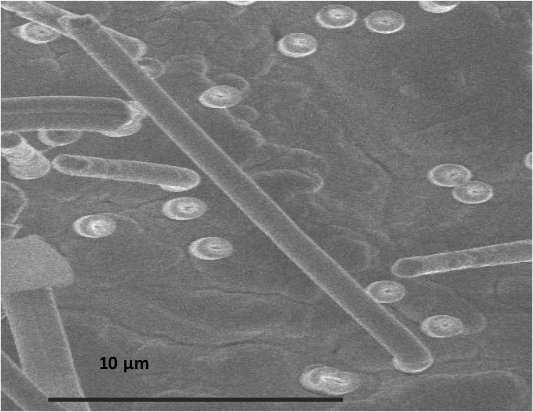
\includegraphics[height=0.35\textwidth]{PC}
			\hfill
			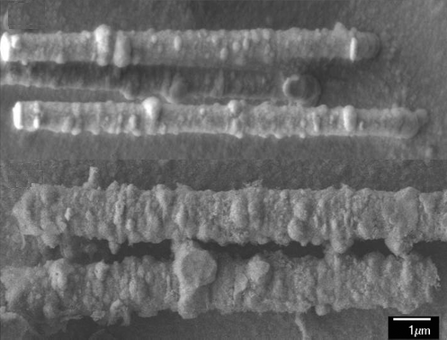
\includegraphics[height=0.35\textwidth]{PET}
			\hfill
			\caption{\textbf{Scanning electron microscope images of metal replica of track-etched PC (left) and PET (right) pores.} The pores were filled with metal and the polymer was completely etched a way, leaving a metal structure that is the inverse image of the pore. The metal was imaged in a scanning electron microscope. While the PC pores are nearly perfectly cylindrical in shape, the PET pores are characterized by rough inhomogenities across their entire surface, punctuated with large local bumps. The large bumps in the images of the metal replicas correspond to equally large cavitities in the PET pore.}
			\label{fig:PCPET}
		\end{figure}
		
		\begin{figure}
			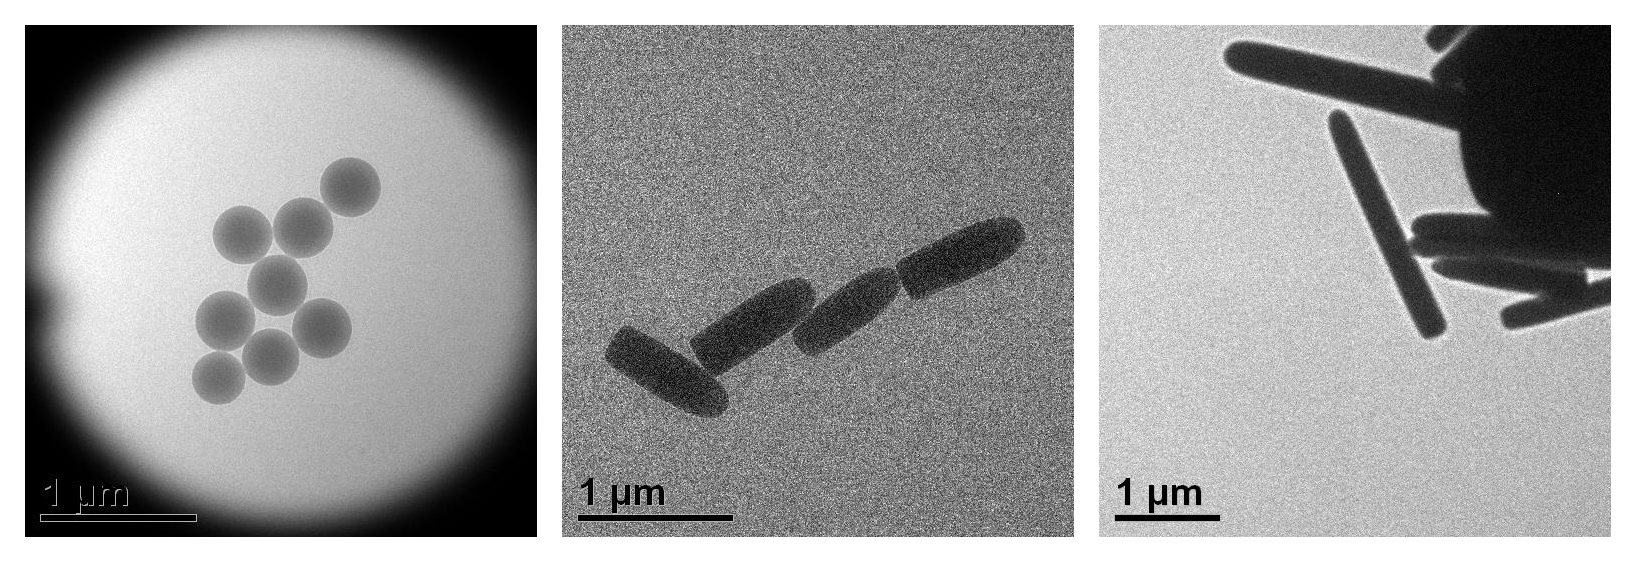
\includegraphics[width=1\textwidth]{particles}
			\caption{\textbf{Transmission electron microscope images of polystyrene beads and silica nanorods.} While the polystyrene beads are nearly perfectly spherical, the silica nanorods are approximately `bullet shaped'. For the purposes of this work, we approximated their shapes as ellipsoids in order to apply equation \ref{eq:dIellipsoid}.}
			\label{fig:particles}
		\end{figure}


	    
		In order to test the method described above for determining the lengths of particles, we performed resistive pulse experiments with single mesopores ranging from $800-\SI{1000}{nm}$ in diameter. The materials used were polyethylene terephthalate (PET), a polymer which is known to have highly irregularly shaped interiors when pores are prepared \textit{via} the track-etch technique, and polycarbonate (PC), another polymer but with no axial inhomogeneities which will act as a control for the method. Figure \ref{fig:PCPET} shows images of both of these types of pores. For the particles, $\SI{280}{nm}$ and $\SI{410}{nm}$ in diameter polystyrene beads (`spheres') were used as the tracer particle, and rods of length $\SI{590}{nm}$, diameter $\SI{210}{nm}$ (`short rods') and $\SI{1920}{nm}$, diameter $\SI{240}{nm}$ (`long rods') were used to test the length measurement protocol; the particles are shown in figure \ref{fig:particles}. Particles were suspended in $\SI{100}{mM}$ KCl solution with $0.5\%$ Tween 80, a surfactant which prevents particle aggregation. The solution was then injected into both sides of a conductivity cell, and a voltage was applied across the pore. The resulting ionic current was sampled at $\SI{10}{kHz}$ and recorded. The polystyrene spheres used had a larger $\zeta-\mathrm{potential}$ than the pore, and therefore they translocated through the pore electrophoretically. On the other hand, the rods had a lower magnitude $\zeta-\mathrm{potential}$ than the pore, and therefore travelled through the pore under electroosmotic convective forces. 
		
	
	\section{Analysis \& Discussion}
	
	
		\begin{figure}
			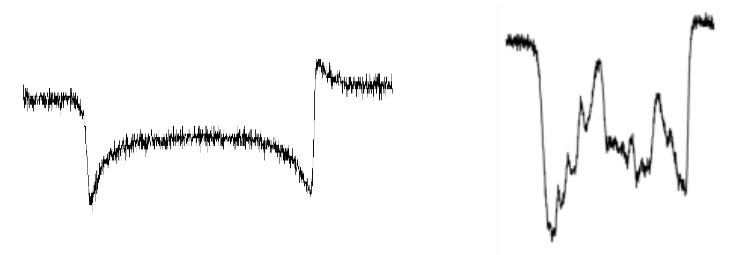
\includegraphics[width=0.5\textwidth]{PCPETevents}
			\caption{\textbf{Resistive pulse events through PC (left) and PET (right) pores.} As expected, the PET events are highly irregular and reflect the interior irregularities of the PET pore itself. On the other hand, the PC pores show no such irregularity. The events show that PC pores have large resistances at the beginning and end, reflecting the narrow, `pinched' diameters at the openings of the pores.}
			\label{fig:PCPETevents}
		\end{figure}

	
	
		Events were extracted from the current time series and studied separately; figure \ref{fig:PCPETevents} shows two events, one from a PC pore and one from a PET pore that are representative of the translocations through each type of pore. In the initial analysis, we looked at the average $\Delta I/I_{p}$ of the beads and rods and compared with the theoretical predictions of Eqs. \ref{eq:dI} and \ref{eq:dIellipsoid}. Figure \ref{fig:dIexp} shows the results for two pores, one $\SI{770}{nm}$ and another $\SI{1200}{nm}$ in diameter. For the two spheres studied, the measured $\Delta I/I_{p}$ was very close to the theoretical prediction (Eq. \ref{eq:dI}). The theoretical predictions were also very close to the measured values for the long rods. However, for both pores the theoretical prediction of the resistive pulse amplitude $\Delta I/I_{p}$ is far off for the short rods: the data shows a nearly 100\% discrepancy, i.e.~ the measured $\Delta I/I_{p}$ is nearly twice its expected value. This significant of a discrepancy is highly unusual, and one of the goals in the paper was to determine its cause. The discrepancy is made even stranger by the fact that the short and long rods are made of the same material, so any material contribution to the discrepancy e.g.~due to large $\zeta-\mathrm{potentials}$ is unlikely. Instead, we hypothesize that this discrepancy is due to their rotational dynamics. Equation \ref{eq:dIellipsoid} predicts that a prolate spheroid (like the rods) will have a larger $\Delta I/I_{p}$ when they are oriented with an off-axis component, but only considers static positioning. A very large rotational speed of the rods could couple to the measured $\Delta I/I_{p}$ amplitude in ways not captured by the equation, for instance by stirring the local solution in such a manner to reduce the local ion mobility. Furthermore, this hypothesis is consistent with the non-observance of the increased $\Delta I/I_{p}$ for the long rods, since at their length of $\sim\SI{1920}{nm}$ they are too large to rotate in even the larger of the two pores ($\SI{1200}{nm}$ in diameter). In any case, the net result is a measured volume for these particles that is approximately $2\times$ larger than their actual volume, which was confirmed with a combination of transmission electron microscopy images and dynamic light scattering. 
		
		The question, however, is how such a large rotation could occur. To answer this question, forces that cause rotation must be considered. In terms of translation (transport), the contributing forces are convection due to electroosmosis, and electrophoresis, as well as passive transport due to diffusion. Similarly, these forces could also contribute to rotational motion of the particles. The estimated rotational diffusion contribution of these rod particles is estimated as $13$ and $\SI{0.8}{rad/s}$ for the short and long rods, respectively. In order for fluid motion to cause rotation, it is necessary to have a non-constant fluid velocity profile on the pore's length. However, because the fluid velocity is due to electroosmosis there will be a nearly constant fluid velocity profile in the pore, which is unlikely to cause significant rotation. On the other hand, the rough undulations in the pore could create axial variations in the electric field; such variations could also lead to a net torque on the particle that causes rotation. In order to estimate the potential magnitude of the rotational velocities of the rods, we considered a simple model where the pore's diameter discontinuously changes from $\SI{1000}{nm}$ to $\SI{1100}{nm}$, a reasonable approximation for the geometries present in our system based on the images of the pores (see Fig. \ref{fig:PET}). Under this model, we calculate the electric field amplitude to differ by a factor of $1.2$ between the two regions. Using the rotational diffusion coefficient of the rods and integrating the electric field differences along the length of the pore, we calculate the angular rotation rate $\omega$ to be $\omega\sim10^{4}$ rad/s. Due to the preceding arguments, it is clear that the largest contribution to the rotation of the rods is from the electric forces. We believe that such a large rotation could make the rods behave as if they are much larger particles.
		
		\begin{figure}
			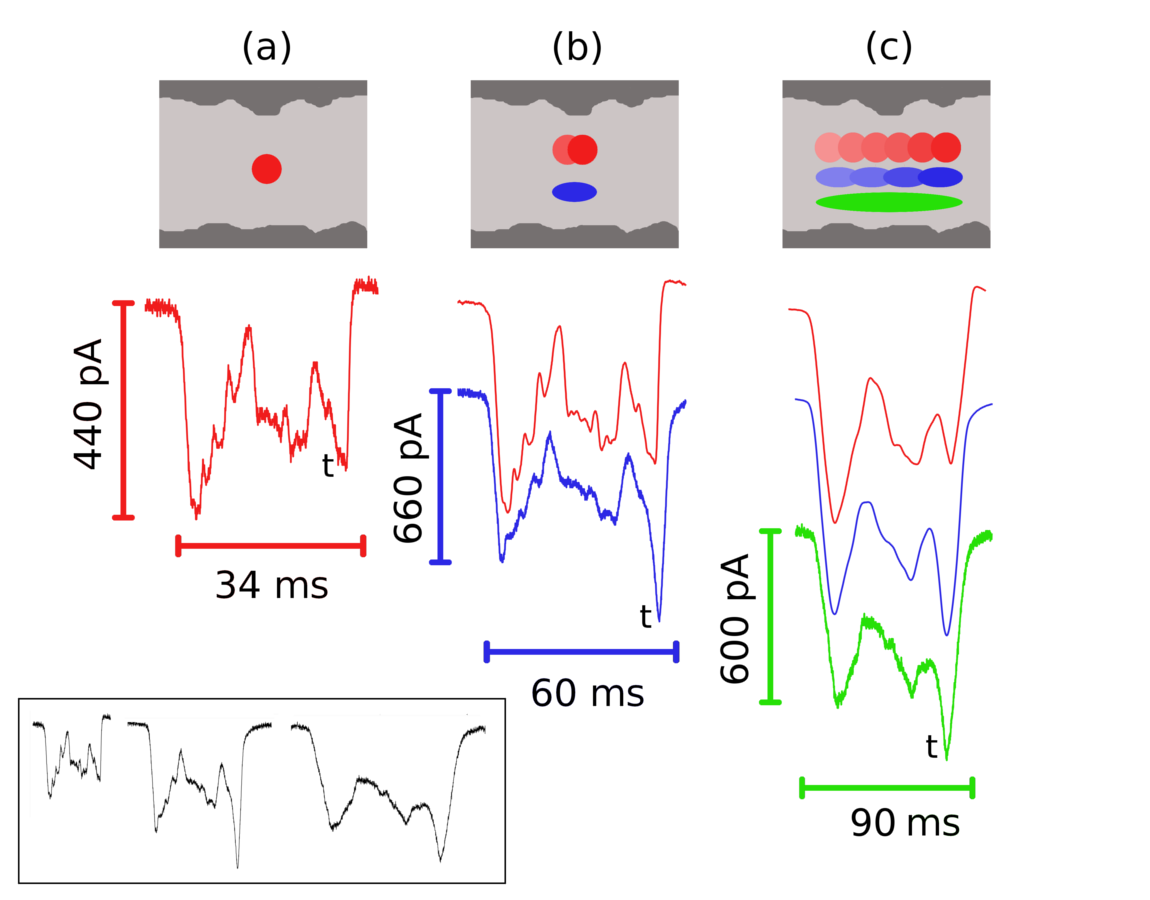
\includegraphics[width=.5\textwidth]{PETevents}
			\caption{\textbf{Resistive pulse events of a $\SI{410}{nm}$ diameter sphere (red), and $\SI{590}{nm}$ (blue) and $\SI{1920}{nm}$ (green) in length rods.} The top row shows a cartoon scheme of the pore with the particles inside its interior. The bottom resistive pulse event in each column corresponds to the raw recorded data; events above this are smoothed \textit{via} the moving average transformation. The bottom left figure shows the raw events on the same scale.}
			\label{fig:PETevents}
		\end{figure}

		
		Figure \ref{fig:PETevents} shows example recorded events for the three types of particles used in this study. A $\SI{410}{nm}$ sphere translocation is shown on the left column in red. Notice the roughness in the event; this roughness has been shown to correspond to the interior irregularities in the pore. Local $\Delta I/I_{p}\left(t\right)$ are large at relatively constricted points, and small at larger cavitated points. The green event in the right column corresponds to the raw resistive pulse signal of a long rod. Notice the difference in structure of the two events; the long rod's event shows some structure, but is missing many of the local minima and maxima that are present in the signal of the short rod. This observation is in agreement with our previous arguments for the smoothing of the pore interior that takes place for long particles. Without making any quantitative arguments, we are able to conclude that the particle corresponding to the green event is longer than the particle corresponding to the red event. In between those two extremes are the short rods in red. The short rods at length $\SI{590}{nm}$ are slightly longer than the spheres which have diameter $\SI{410}{nm}$, but due to their rotation it is not entirely obvious whether they should image the pore with the same resolution as the spheres. Looking at the results, the signals of the short rod and sphere are much more similar than the long rod and the sphere, but some local structure is still unresolved for the short rods. 
		
		In order to test the hypothesis that long particles behave as a moving average of shorter particles, we calculated moving averages of the spheres and the short rods. The time over which the moving average was calculated corresponded to the duration in time over which the particle travelled a distance equal to the length of the longer particle with which it is being compared. We determined the average velocity of a particle from the total translocation distance (the known length of the pore, $L'=L-D$) and the translocation duration measured from the RP signal, $\Delta T$. The velocity is then $v=L'/\Delta t$. The moving average window then has length (in time) of $\Delta t=v/l$, which corresponds to a window of $N=f\times\Delta t$ data points in length. The transformation then from the raw signal $I_{i}$ to the averaged signal $I'_{i}$ is
		
		
		\begin{equation} \label{eq:movingavg}
			I'_{i}=\frac{1}{N}\sum_{j=-N/2}^{N/2}I_{j}.
		\end{equation}
		
		This moving average process was performed on the spheres and on the short rods. The red signal in the middle column corresponds to the moving average of the spheres over the length of the short rods, and the red signal in the right column corresponds to the moving average of the spheres over the length of the long rods. Finally, the moving average of the short rods over the length of the long rods is the blue signal in the right column. Qualitatively, we see that the moving average process, which is physically motivated by the equations for the resistance of small particles in series, recovers the appearance of the signals of longer particles. 
		
		\begin{figure}
			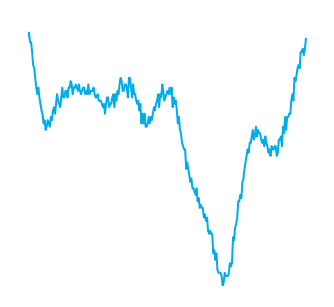
\includegraphics[width=0.5\textwidth]{longevent.png}
			\caption{\textbf{Resistive pulse signal of a single long rod passing through a PET pore.} The variation in the amplitude of the current signals that the pore has an inhomogeneous interior shape.}
			\label{fig:longevent}
		\end{figure}

		
		\begin{figure}
			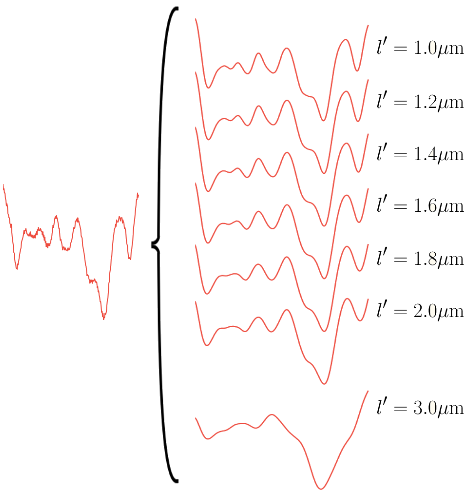
\includegraphics[width=0.5\textwidth]{experimentaldtwfits.png}
			\caption{\textbf{Resistive pulse signal of a single short rod passing through a PET pore alongside many instances of the moving average transformation performed on the signal for different length intervals.} As the length interval is increased, the finer structure of the resistive pulse signal is smoothed over. For the greatest length measured, many of the features prominent in the raw signal have disappeared..}
			\label{fig:experimentaldtwfits}
		\end{figure}
		
		
		\begin{figure}
			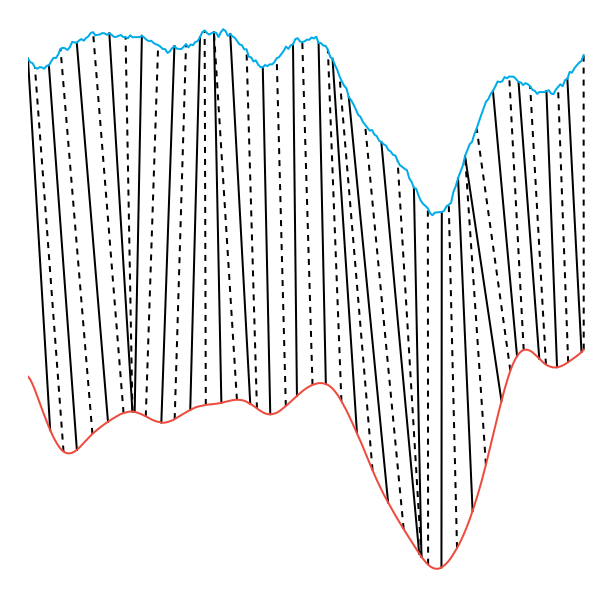
\includegraphics[width=0.5\textwidth]{experimentaldtwfit.png}
			\caption{\textbf{Raw resistive pulse signal of a single long rod matched with the signal of a short rod that has been transformed via the moving average process.} The aligned points were determined by the dynamic time warping algorithm, and the particular transformation shown was the one that minimized the difference between the two signals, also determined by the dynamic time warping algorithm.}
			\label{fig:experimentaldtwfit}
		\end{figure}
		
		
		In order to measure the lengths of the long rods, we performed the dynamic time warping technique described in the preceding section. Figure \ref{fig:longevent} shows a single instance of a long rod passing through a PET pore. Figure \ref{fig:experimentaldtwfits} shows a shorter rod particle averaged over many different length intervals. As the short rod is averaged over a greater length interval, it continuously transforms into a shape that bears a stronger resemblance to the signal of the long rods. Of all the fits calculated in Fig. \ref{fig:experimentaldtwfits}, the correct length is determined by the fit with the smallest cost as determined by dynamic time warping. An example resistive pulse signal of a long rod and a shorter rod that has been transformed \textit{via} the moving average equation is shown in Fig. \ref{fig:experimentaldtwfit}. Finally, after performing the moving average and dynamic time warping minimization approach described above, we were able to determine the expected lengths of the long rods according to this algorithm. Figure \ref{fig:dtwfit} shows a plot of histograms of the lengths as determined by this approach, alongside a Gaussian fit to the histogram, and a Gaussian distribution that shows the actual distribution of hte lengths of the long particles as determined by electron microscopy images. The figure reveals that, in this case, the dynamic time warping algorithm is able to successfully recover the real distribution of the known lengths relatively accurately.
		
		
		\begin{figure}
			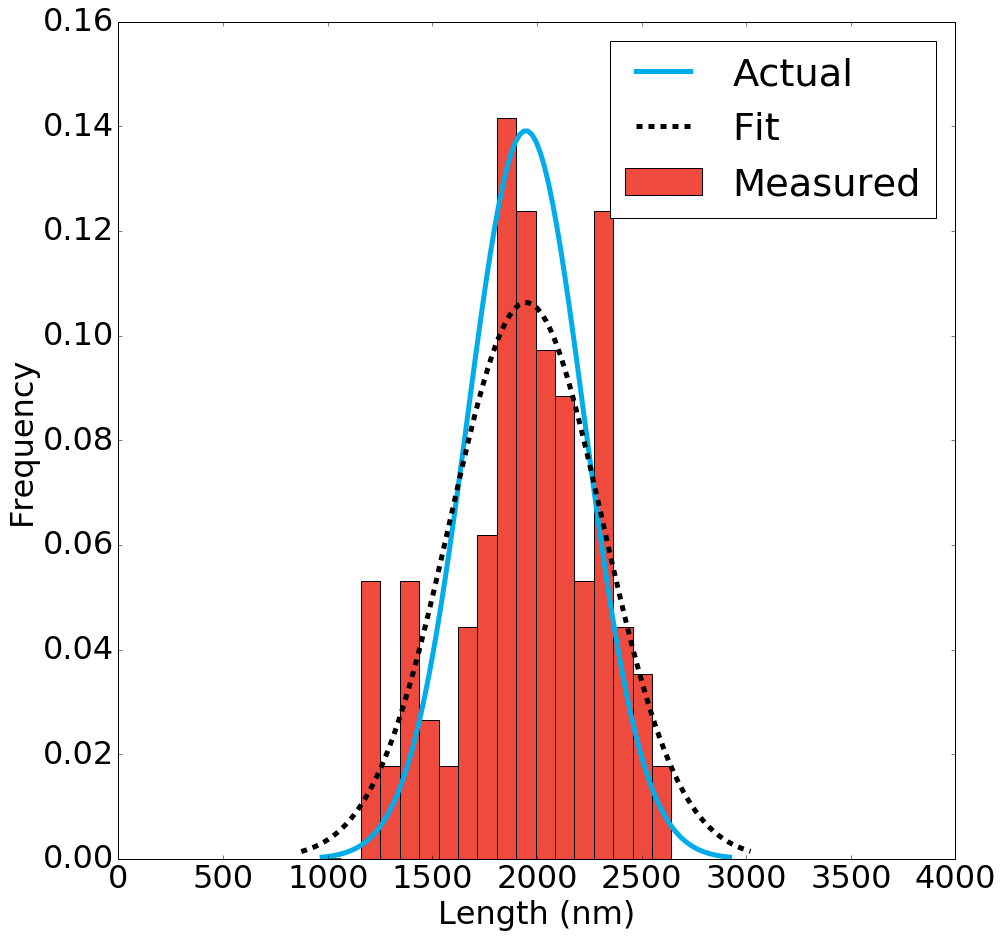
\includegraphics[width=0.5\textwidth]{dtwfit.png}
			\caption{\textbf{Histogram of particle length as determined by dynamic time warping along with the actual distribution of sizes determined by electron microscopy imaging.} A normal distribution is fit to the histogram of particle lengths as determined by dynamic time warping and shown to be in good agreement with the expected distribution.}
			\label{fig:dtwfit}
		\end{figure}
		
	\section{Conclusions}
		In summary, we presented resistive pulse experiments performed with spherical and non-spherical particles in two types of pores, those with smooth interiors (PC) and rough interiors (PET). We devised a protocol for measuring the lengths of long particles by taking advantage of the rough interiors of PET pores, which reflect in the measured resistive pulse signals of all the particles. Longer particles displace a greater distance along the pore's length, and therefore their signals are a more smoothed version of the signals of shorter particles. This smoothing attribute can be recovered by taking the moving averages of shorter particles. By performing moving averages for many different particle lengths and measuring the similarity between the raw signal of the long particles with each of the transformed signals of the shorter particles, we were able to determine the length distribution of the long particles used in experiments. Dynamic time warping was used as a means of effectively comparing the similarity of the signals of the two particles. While the general premise of the `smoothing' of the resistive pulse signals by long particles compared to short particles is convincingly established, more research must be performed on the hybrid moving average-dynamic time warping method. The protocol was only tested for a small number of pores and only two types of particles, short and long rods. In the future, an ideal experiment could be performed with small spherical beads and rods of various unknown lengths. The experiments and analysis would be performed in a blind fashion, and only after the analysis is complete would the true length distribution of the long rods be revealed. If the length measurement protocol survives this blind study, it would prove to be a very effective means of determining the lengths of small particles.
		
		Additionally, a likely unrelated phenomena was discovered where short, aspherical particles created far greater (up to 2x) resistive pulse amplitudes than predicted by the well-established classical equations. The exact reason for this effect is still unclear, however we laid out arguments that explain rotational dynamics as a likely culprit. We reasoned from our studies that an extremely rapid rate of rotation could effectively increase the radius of the particle, possibly by disturbing the local solution and decreasings its conductivity. Such rotations would not be possible for the longer rods due to their prohibitively long lengths compared ot the diameter of the pore. However, more investigation must be performed in order to convincingly show that not only do short rod like objects deviate strongly from the classical equations, but also that rotational dynamics is the culprit. Additional experiments must be performed with a larger variety of short rods to show that the effect is general and not limited to the rods used in this study. Furthermore, experiments could be designed in such a way as to retard the rods' rotations, perhaps by using smaller pores or solution with an increased viscosity.

	
	
		
		
		
	

	




%%% Local Variables: ***
%%% mode: latex ***
%%% TeX-master: "thesis.tex" ***
%%% End: ***
